\documentclass[conference]{IEEEtran}
\usepackage{cite}
\usepackage{amsmath,amssymb,amsfonts}
\usepackage{amsthm}
\usepackage{graphicx}
\usepackage{xcolor}
\usepackage{booktabs}
\usepackage{array}
\usepackage{multirow}
\usepackage{url}
\usepackage{tikz}
\usetikzlibrary{arrows.meta,positioning}
\usepackage{pgfplots}
\pgfplotsset{compat=1.17}

\newtheorem{proposition}{Proposition}

% Two authors per row (IEEE individual author blocks).
\makeatletter
\newcommand{\linebreakand}{%
  \end{@IEEEauthorhalign}
  \hfill\mbox{}\par
  \mbox{}\hfill\begin{@IEEEauthorhalign}
}
\makeatother
\newcommand{\RQ}[1]{\textbf{RQ#1}}

\begin{document}

\title{Who Writes the Evidence? Counterparty-Confirmed Track Records in MentorConnect}

\author{\IEEEauthorblockN{Himani Pilankar}
\IEEEauthorblockA{\textit{Department of Computer Engineering}\\
\textit{Sardar Patel Institute of Technology}\\
Mumbai, India}
\and
\IEEEauthorblockN{Tithi Talele}
\IEEEauthorblockA{\textit{Department of Computer Engineering}\\
\textit{Sardar Patel Institute of Technology}\\
Mumbai, India}
\linebreakand
\IEEEauthorblockN{Chetan Wankhede}
\IEEEauthorblockA{\textit{Department of Computer Engineering}\\
\textit{Sardar Patel Institute of Technology}\\
Mumbai, India}
\and
\IEEEauthorblockN{Dr. Sudhir Dhage}
\IEEEauthorblockA{\textit{Department of Computer Engineering}\\
\textit{Sardar Patel Institute of Technology}\\
Mumbai, India}}

\maketitle

\begin{abstract}
On peer-mentoring platforms, the candidate being ranked often writes the records used to rank them: mentors log their own sessions and, in many systems, their own ratings. We study \emph{evidence gating}, a design rule under which a session record may influence a mentor's rank only if a verified mentee created or confirmed it and authored its feedback. We state the rule as write-time invariants, show that mentor-only session records then cannot affect any ranking, characterise how much credit a colluding record can earn, and implement the rule in MentorConnect, an institute mentoring platform. Running the platform's ranking function on simulated campuses with hidden ground truth and three manipulation strategies, we compare nine rankers over 20 seeds with Holm-corrected paired tests. Trusting all logged history lowers NDCG@10 from 0.716 (content-only ranking) to 0.630 and gives manipulators 32.9\% of top-10 slots against a 14.7\% pool share. With the scorer fixed, and even when honest unconfirmed sessions are reported truthfully, the gate raises NDCG@10 by 0.033 and Precision@5 by 0.071 and cuts manipulator exposure from 26.4\% to 19.1\% in all 20 seeds ($p<0.001$). Compared with content-only ranking, gated history raises Precision@5 by 7\% while manipulator exposure stays within $\pm2.5$ percentage points (equivalence test, $p=0.006$). Extending the gate to count at most one record per mentee further cuts colluder exposure by 22\% and improves every accuracy metric.
\end{abstract}

\begin{IEEEkeywords}
recommender systems, reputation systems, shilling attacks, verified feedback, peer mentoring, educational technology
\end{IEEEkeywords}

\section{Introduction}
Peer mentoring is among the most studied interventions for student persistence, yet reviews spanning three decades report the same gaps: inconsistent definitions, weak outcome measurement and programmes that depend on who happens to know whom \cite{jacobi1991,gershenfeld2014}. Institutes increasingly run mentoring through web platforms, where a recommender that matches a student's learning needs to mentors' skills is the natural first feature \cite{manouselis2011,pham2023}. Content matching alone cannot tell a capable mentor from one who merely lists the right skills, so platforms add \emph{track-record} signals such as ratings, session counts, completion rates and recency, the standard hybrid of content and behavioural evidence \cite{burke2002}.

Track records carry a vulnerability that is specific to mentoring. In product recommendation, consumers rate items. On a mentoring platform the session log is often written by the mentor, who is also the candidate being ranked. A mentor who logs sessions that never happened, or rates them five stars, mounts a profile-injection (``shilling'') attack \cite{lam2004,mobasher2007} without creating a single fake account. Detection-based defences classify suspicious rating profiles after the fact \cite{gunes2014,si2020}, and reputation systems handle self-promotion mainly through identity and Sybil controls \cite{hoffman2009,cheng2005}. Neither addresses a platform on which the ratee authors the interaction log itself.

Restricting reviews to verified customers is an established remedy for consumer reviews: hotel reviews on Expedia, which require a booking, are less promotional than those on TripAdvisor \cite{mayzlin2014}, and optional purchase verification improves rating quality \cite{kokkodis2022}. We study the transfer of this principle to peer-mentor ranking, where the ranked party writes the log and histories are typically sparse. We call the resulting rule \emph{evidence gating}: a record may influence a mentor's rank only if the mentee created or confirmed it and wrote its feedback. We ask:
\begin{itemize}
\item \RQ{1}: Does ranking on unverified history make a mentor recommender less accurate and easier to manipulate than ignoring history?
\item \RQ{2}: Does evidence gating remove that damage, under a fair comparison, and is the effect due to the gate or to Bayesian shrinkage?
\item \RQ{3}: Which manipulation strategies does the gate stop, can collusion be bounded further, and how sensitive are the conclusions to confirmation rate, collusion strength and history depth?
\end{itemize}

Our contributions are as follows.
\begin{enumerate}
\item \textbf{A formal statement of evidence gating} as write-time invariants on session records, with the guarantee it provides against self-reporting and an exact account of the credit a colluding record still earns (Section~\ref{sec:method}).
\item \textbf{An implementation} in MentorConnect, a deployed institute mentoring platform, including a mentee confirmation workflow and per-list recommendation logging (Section~\ref{sec:system}).
\item \textbf{A controlled study} that uses the platform's ranking function on simulated campuses with hidden ground truth. It compares nine rankers over 20 seeds with Holm-corrected paired tests, includes a fair ungated baseline and a shrinkage ablation, and tests a one-record-per-mentee extension against collusion (Sections~\ref{sec:setup}--\ref{sec:results}).
\end{enumerate}

\section{Related Work}
\label{sec:related}
\textbf{Mentor and people recommendation.} Recommending people differs from recommending items: both sides must be willing, and success depends on the interaction that follows \cite{terveen2005}. Reciprocal recommenders model both sides' preferences \cite{pizzato2010}. Mentor--mentee matching has been approached with fuzzy profile matching \cite{pham2023} and with two-sided matching algorithms, where participants can manipulate their stated preferences \cite{haas2019}. These systems rank on profile and preference fit and do not use track records; we study what happens when they do.

\textbf{Attacks on recommenders.} Shilling attacks inject fake profiles to promote or demote targets \cite{lam2004}. Attack models and robustness have been analysed in depth \cite{mobasher2007,gunes2014}, and surveys catalogue detectors built on rating statistics, clustering and deep learning \cite{si2020,sundar2020}. Optimised poisoning attacks evade such detectors by mimicking normal users \cite{li2016,fang2018}. Trust-aware recommenders weight \emph{raters} by inferred trust \cite{massa2007}. Evidence gating instead constrains, at write time, which records exist as evidence, and so needs neither labelled attacks nor a model of the attacker.

\textbf{Reputation systems.} Reputation systems aggregate feedback about past behaviour to support trust between strangers \cite{resnick2000}, and Bayesian formulations such as the beta reputation system \cite{josang2002} motivate our shrinkage. Known attacks include self-promotion, collusion and Sybil identities \cite{hoffman2009,douceur2002,cheng2005}. Field and laboratory evidence shows that verification reduces promotional reviewing \cite{mayzlin2014,kokkodis2022}, and that two-sided feedback invites reciprocity and fear of retaliation \cite{bolton2013,fradkin2021}. We apply the verified-customer principle where the ratee controls the log, and measure its effect on ranking rather than on review volume.

\section{Problem Formulation and Threat Model}
\label{sec:problem}
A student $s$ has learning needs $N_s$. Each mentor $m$ has hidden expertise $E_m$ and hidden mentoring quality $q_m\in[0,1]$. The platform observes a profile and a set of session records $R_m$. A record $r$ has a mentor, a mentee, a timestamp, a status $\sigma_r\in\{\text{pending},\text{confirmed},\text{disputed}\}$ and optional feedback: a rating $\rho_r\in\{1,\dots,5\}$, an outcome (resolved or not), a follow-up flag and a would-recommend flag. The recommender should rank highly, for each student, the mentors who cover $N_s$ and have high $q_m$.

\textbf{Adversary.} A manipulator is a low-quality mentor who wants more top-$k$ exposure. We consider three strategies: a \emph{stuffer} lists popular skills and interests they do not have (a content attack); an \emph{inflator} logs many sessions with self-assigned five-star, resolved feedback that no mentee confirms (self-reporting); and a \emph{colluder} has real friends confirm fabricated five-star sessions (collusion, which passes any confirmation step). Only institute-verified students can confirm evidence (I5 below), so a mentor cannot mint confirming identities \cite{douceur2002}.

Coerced confirmations, compromised accounts and signals other than session records are outside the scope of this paper.

\section{Evidence-Gated Reputation}
\label{sec:method}
\subsection{The Gate}
Only the gated set
\begin{equation}
G_m=\{\,r\in R_m:\sigma_r=\text{confirmed}\,\}
\label{eq:gate}
\end{equation}
may influence $m$'s score. Confirmation is meaningful because the platform enforces five invariants.
\begin{enumerate}
\item[I1:] \emph{Counterparty confirmation.} Only the mentee of $r$ can set $\sigma_r$ to confirmed; a session the mentee logs is confirmed on creation.
\item[I2:] \emph{Counterparty authorship.} Every feedback field of $r$ is written by the mentee; values submitted by the mentor are discarded.
\item[I3:] \emph{Immutability.} After confirmation, no field used for ranking can be edited, except that the mentee may mark a follow-up as completed.
\item[I4:] \emph{Disputability.} The mentee may dispute a mentor-logged record instead of confirming it, which excludes it permanently.
\item[I5:] \emph{Verified counterparty.} A confirmation counts only if the mentee is an email-verified current student of the institute; other confirmations are kept in history but carry no weight.
\end{enumerate}

\subsection{Quality, Activity and Responsiveness}
Let $n$ be the number of rated records in $G_m$, with mean rating $\bar\rho$. Following the beta reputation system \cite{josang2002}, the mean is shrunk toward a neutral prior $\mu_0=3.5$ with strength $k=5$ and weighted by a confidence term $c$:
\begin{equation}
\tilde\rho=\frac{k\mu_0+n\bar\rho}{k+n},\qquad c=\frac{n}{n+k}.
\label{eq:shrink}
\end{equation}
Let $\kappa$ be the share of records in $G_m$ that were resolved or followed up, and $\omega$ the would-recommend rate smoothed toward $0.7$. Quality is
\begin{equation}
Q_m=(1-\lambda)\left(0.6\,c\,\frac{\tilde\rho}{5}+0.4\,\kappa\right)+\lambda\,\omega ,
\label{eq:quality}
\end{equation}
with $\lambda=0.2$ when would-recommend answers exist and $\lambda=0$ otherwise. Activity rewards the volume and recency of gated records,
\begin{equation}
A_m=\min\!\left(1,\;\frac{|G_m|}{120}+\frac12\max\!\left(0,1-\frac{\Delta t}{90}\right)\right),
\label{eq:activity}
\end{equation}
where $\Delta t$ is the number of days since the last record in $G_m$. Responsiveness is the share of mentorship requests that $m$ accepted, smoothed with a Beta(2,2) prior.

\subsection{Ranking}
Each eligible mentor receives a weighted sum of normalised features,
\begin{equation}
S(s,m)=\sum_{j} w_j f_j(s,m),\qquad \textstyle\sum_j w_j=1 ,
\label{eq:score}
\end{equation}
clipped to $[0,1]$. The fit features (68.4\% of the weight) are need coverage, profile-text similarity, topic overlap, project relevance, department, year gap, availability, profile completeness, cluster fit and a primary-cluster bonus. The evidence features (31.6\%) are $Q_m$ (13.5\%), $A_m$ (8.3\%), a mentoring-evidence term derived from achievements and session volume (6.0\%), and responsiveness (3.8\%). Each list is returned with per-feature contributions, so every recommendation can be explained.

\subsection{Guarantees}
\begin{proposition}[Self-report invariance]
\label{prop:invariance}
Let $X$ be a set of session records created by mentor $m$ and never confirmed by their mentees. Adding $X$ to the platform leaves $S(s,m')$ unchanged for every student $s$ and every mentor $m'$, and hence leaves every ranking unchanged.
\end{proposition}
\begin{proof}
Session records enter $S$ only through the gated sets (Eqs.~\eqref{eq:gate}--\eqref{eq:activity}). By I1, records in $X$ remain pending, and by I5 they cannot be confirmed through accounts $m$ creates, so no gated set changes. By I2 and I3, $m$ cannot alter the ranked fields of records already in $G_m$.
\end{proof}
The proposition follows directly from the invariants, which makes the guarantee explicit and testable at the API level.

\begin{proposition}[Bounded rating credit]
\label{prop:collusion}
For a mentor with no other history, $n$ confirmed records rated 5 contribute exactly
\begin{equation}
\Delta(n)=0.6\,\frac{n\,(k\mu_0+5n)}{5\,(n+k)^2}
\end{equation}
to the rating term of Eq.~\eqref{eq:quality}, against $0.6$ for any $n\ge1$ without shrinkage.
\end{proposition}
\begin{proof}
Substitute $\bar\rho=5$ into Eq.~\eqref{eq:shrink} and form $0.6\,c\,\tilde\rho/5$.
\end{proof}
With $k=5$ and $\mu_0=3.5$, $\Delta(1)=0.075$, one eighth of the unshrunk value. The bound covers only the rating term, however. Completion rate and recency are not shrunk, so one colluding, ``resolved'' record raises a new mentor's score $S$ by about $0.115$, of which the rating term contributes only $0.008$. We therefore complement shrinkage with a structural rule, counting at most one record per mentor--mentee pair, so that a colluder's gated history is bounded by the number of distinct accomplices.

\section{System Implementation}
\label{sec:system}
MentorConnect is a web platform (Node.js, Express, MongoDB, Socket.IO) with one-time-password (OTP) verified accounts, mentorship requests, chat and achievement certificates. Ranking runs in a separate Python FastAPI service. In the deployed service, every engine version receives pre-aggregated statistics computed over confirmed sessions only. When a mentor logs a session, the mentee is notified and either confirms it, entering their own feedback, or disputes it (Fig.~\ref{fig:gate}). Only confirmed records reach the ranker and the ledger that issues certificates, so certificates cannot be inflated by self-reporting either. The platform also serves external and alumni users; their confirmations are stored but, by I5, flagged at write time as non-evidence and excluded from ranking, contribution points and certificates. An end-to-end test suite of 34 checks verifies I1--I5 against the running API.

\begin{figure}[t]
\centering
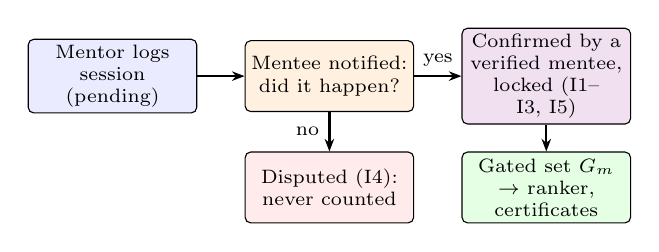
\begin{tikzpicture}[every node/.style={font=\scriptsize, align=center},
  box/.style={draw, rounded corners=2pt, minimum height=9mm, inner sep=2pt, text width=20mm},
  arr/.style={-{Stealth[length=1.6mm]}, thick}]
\node[box, fill=blue!8] (log) {Mentor logs\\session (pending)};
\node[box, fill=orange!12, right=6mm of log] (q) {Mentee notified:\\did it happen?};
\node[box, fill=violet!12, right=6mm of q] (c) {Confirmed by a\\verified mentee,\\locked (I1--I3, I5)};
\node[box, fill=red!8, below=5mm of q] (d) {Disputed (I4):\\never counted};
\node[box, fill=green!10, right=6mm of d] (e) {Gated set $G_m$\\$\rightarrow$ ranker,\\certificates};
\draw[arr] (log) -- (q);
\draw[arr] (q) -- node[above]{yes} (c);
\draw[arr] (q) -- node[left]{no} (d);
\draw[arr] (c) -- (e);
\end{tikzpicture}
\caption{Session life cycle under evidence gating. Only records the mentee confirmed and annotated enter $G_m$.}
\label{fig:gate}
\end{figure}

\section{Experimental Setup}
\label{sec:setup}

\begin{table*}[t]
\centering
\caption{Main results at a 15\% manipulator rate (mean $\pm$ sample standard deviation over 20 seeds). Manip@10, the per-strategy columns and New@10 are percentages of top-10 slots. Pool shares: manipulators 14.7\% (stuffers 5.3\%, inflators 4.7\%, colluders 4.7\%), honest newcomers 19.3\%.}
\label{tab:main}
\footnotesize
\setlength{\tabcolsep}{4pt}
\renewcommand{\arraystretch}{1.12}
\begin{tabular}{lcccc ccc cc}
\toprule
 & \multicolumn{4}{c}{Accuracy and overall manipulation} & \multicolumn{3}{c}{Manip@10 by strategy} & \multicolumn{2}{c}{Exposure} \\
\cmidrule(lr){2-5}\cmidrule(lr){6-8}\cmidrule(lr){9-10}
Ranker & NDCG@10 & P@5 & MRR & Manip@10 & Stuffer & Inflator & Colluder & New@10 & Gini \\
\midrule
Random & 0.171 $\pm$ 0.009 & 0.144 $\pm$ 0.013 & 0.321 $\pm$ 0.024 & 14.3 $\pm$ 0.9 & 5.3 & 4.6 & 4.4 & 19.5 & 0.204 \\
Popularity & 0.118 $\pm$ 0.028 & 0.051 $\pm$ 0.051 & 0.154 $\pm$ 0.089 & 70.5 $\pm$ 10.0 & 0.0 & 65.0 & 5.5 & 0.0 & 0.933 \\
Content-only & 0.716 $\pm$ 0.014 & 0.545 $\pm$ 0.047 & 0.735 $\pm$ 0.053 & 18.3 $\pm$ 1.7 & 9.2 & 4.6 & 4.5 & 18.8 & 0.287 \\
\midrule
V1 (all logs count) & 0.630 $\pm$ 0.024 & 0.445 $\pm$ 0.044 & 0.594 $\pm$ 0.039 & 32.9 $\pm$ 2.8 & 6.4 & 16.8 & 9.8 & 2.0 & 0.546 \\
V3-ungated, as logged & 0.657 $\pm$ 0.022 & 0.480 $\pm$ 0.041 & 0.632 $\pm$ 0.041 & 29.5 $\pm$ 2.5 & 5.1 & 15.2 & 9.1 & 2.2 & 0.510 \\
V3-ungated, truthful & 0.678 $\pm$ 0.020 & 0.513 $\pm$ 0.042 & 0.683 $\pm$ 0.050 & 26.4 $\pm$ 2.6 & 5.0 & 13.4 & 8.0 & 1.4 & 0.493 \\
V3-no-shrink (ablation) & 0.724 $\pm$ 0.017 & 0.615 $\pm$ 0.044 & 0.791 $\pm$ 0.040 & 18.0 $\pm$ 2.2 & 5.5 & 3.0 & 9.5 & 0.8 & 0.505 \\
\textbf{V3} (gated) & 0.711 $\pm$ 0.017 & 0.585 $\pm$ 0.047 & 0.772 $\pm$ 0.048 & 19.1 $\pm$ 2.4 & 6.0 & 3.1 & 9.9 & 2.5 & 0.488 \\
\textbf{V3 + per-mentee cap} & 0.723 $\pm$ 0.017 & 0.604 $\pm$ 0.047 & 0.803 $\pm$ 0.050 & 17.2 $\pm$ 2.2 & 6.2 & 3.3 & 7.7 & 2.6 & 0.482 \\
\bottomrule
\end{tabular}
\end{table*}

\subsection{Why Simulation}
Evaluating robustness requires knowing which mentors are good and which are manipulating, and live platforms reveal neither. Live logs are also confounded by the recommender that produced them \cite{chaney2018}. We therefore follow the simulation methodology standard in attack research \cite{mobasher2007}: we generate campuses with hidden ground truth and pass only platform-visible data to the platform's ranking function, unmodified. Three differences from deployment apply. The simulator passes per-session records, whereas production passes pre-aggregated confirmed-only statistics. No mentorship or achievement data are simulated, so responsiveness is constant ($0.5$) and the mentoring-evidence term reduces to session volume. And V1 reconstructs the legacy behaviour of counting every logged session.

\subsection{Campus Generator}
Each campus has 150 mentors, 100 students and ten topic areas. Honest mentors draw $q_m\sim\mathrm{Beta}(5,2)$ and one to three expertise topics, and their profiles list skills from those topics plus, with probability 0.2, an unrelated popular skill. Session volume is log-normal and only weakly related to quality; 22.7\% of honest mentors have no history. Each honest session, dated within the last 180 days, is confirmed with probability $p_c=0.65$. Confirmed sessions carry J-shaped ratings \cite{hu2006}, and their outcomes, follow-ups and would-recommend answers depend on $q_m$. Manipulators draw $q_m\sim\mathrm{Beta}(2,4)$, have organic histories generated in the same way, and make up 15\% of mentors, assigned in rotation to the three strategies. Stuffers add ten popular skills and five topics. Inflators add 20--40 self-logged five-star sessions, and colluders 4--8 confirmed five-star sessions from two friends, all dated within 60 days, which gives attackers a recency advantage.

\subsection{Relevance and Metrics}
The graded gain of mentor $m$ for student $s$ is $|N_s\cap E_m|/|N_s|\cdot q_m$. A mentor is \emph{relevant} if the mentor covers at least one need, is honest and has $q_m\ge0.65$. We report normalised discounted cumulative gain (NDCG@10) \cite{jarvelin2002} with graded gains, which credits manipulators only for their low true quality. We also report precision at 5 (P@5) and mean reciprocal rank (MRR), which treat manipulators as irrelevant. For exposure, we report Manip@10, the share of top-10 slots held by manipulators, overall and per strategy; New@10, the share held by honest newcomers; and the Gini coefficient of top-10 exposure across mentors.

\subsection{Rankers}
Besides \emph{Random} and \emph{Popularity} (most logged sessions), we compare the following rankers.
\begin{itemize}
\item \emph{Content-only}: V3 without history (profile fit only).
\item \emph{V1}: the legacy engine, in which every log counts.
\item \emph{V3-ungated, as logged}: V3 fed every record as if confirmed. This removes I1 and I2 together, so honest unconfirmed sessions carry no feedback.
\item \emph{V3-ungated, truthful}: the same, except that honest unconfirmed sessions carry the feedback the mentee would have given, drawn from the same model. This is the fair test of the gate.
\item \emph{V3-no-shrink}: V3 with raw averages ($c=1$, $\tilde\rho=\bar\rho$, unsmoothed $\omega$), which isolates shrinkage.
\item \emph{V3}: evidence-gated, as deployed.
\item \emph{V3 + per-mentee cap}: V3 counting only the latest confirmed record per mentor--mentee pair.
\end{itemize}

\subsection{Protocol}
The main condition uses 20 seeds; all rankers see the same campus within a seed, so we pair by seed. For each metric we compare V3 with each alternative using paired $t$-tests and Wilcoxon signed-rank tests, with Holm correction applied separately to each test within a family of comparisons. We report 95\% confidence intervals and paired effect sizes $d_z$. The four-fold history condition uses ten seeds, and the remaining sensitivity settings use five and are indicative. Code and results are released with the platform.

\section{Results}
\label{sec:results}

\begin{table}[t]
\centering
\caption{Paired differences, V3 minus each alternative, over 20 seeds. $\Delta$Manip and $\Delta$New are in percentage points. $^{*}$: Holm-corrected $p<0.05$ under both the paired $t$-test and the Wilcoxon test.}
\label{tab:tests}
\footnotesize
\setlength{\tabcolsep}{3pt}
\renewcommand{\arraystretch}{1.12}
\resizebox{\columnwidth}{!}{%
\begin{tabular}{lccccc}
\toprule
V3 vs. & $\Delta$NDCG@10 & $\Delta$P@5 & $\Delta$MRR & $\Delta$Manip & $\Delta$New \\
\midrule
V1 & $+0.081^{*}$ & $+0.139^{*}$ & $+0.178^{*}$ & $-13.8^{*}$ & $+0.4^{*}$ \\
Ungated, as logged & $+0.055^{*}$ & $+0.105^{*}$ & $+0.140^{*}$ & $-10.4^{*}$ & $+0.2^{*}$ \\
Ungated, truthful & $+0.033^{*}$ & $+0.071^{*}$ & $+0.089^{*}$ & $-7.3^{*}$ & $+1.1^{*}$ \\
No-shrink & $-0.012^{*}$ & $-0.031^{*}$ & $-0.019^{*}$ & $+1.1^{*}$ & $+1.6^{*}$ \\
Per-mentee cap & $-0.011^{*}$ & $-0.019^{*}$ & $-0.031^{*}$ & $+1.9^{*}$ & $-0.1$ \\
Content-only & $-0.005$ & $+0.040^{*}$ & $+0.037^{*}$ & $+0.8$ & $-16.4^{*}$ \\
\bottomrule
\end{tabular}}
\end{table}

\subsection{RQ1: Unverified History Is Harmful}
Trusting every logged session makes ranking worse than ignoring history (Table~\ref{tab:main}). V1 lowers NDCG@10 from 0.716 (Content-only) to 0.630 and P@5 from 0.545 to 0.445, and gives manipulators 32.9\% of top-10 slots against their 14.7\% pool share. Both differences hold in all 20 seeds (paired $t$-test $p<10^{-12}$, $|d_z|>4$). The damage comes from the data, not from V1's weights: the V3 scorer fed ungated logs also falls below Content-only, to 0.657 NDCG@10 as logged and 0.678 with truthful reports. Popularity hands 70.5\% of the top~10 to manipulators.

\subsection{RQ2: The Gate Removes the Damage}
The fair test of the gate compares V3 with V3-ungated, truthful: the two use the same scorer and the same honest feedback, and differ only in whether unconfirmed records count. The gate raises NDCG@10 by 0.033 (95\% CI $[0.026,0.039]$), P@5 by 0.071 and MRR by 0.089, and cuts manipulator exposure from 26.4\% to 19.1\%. V3 is better on every accuracy metric in each of the 20 seeds (Table~\ref{tab:tests}). Against the as-logged ungated baseline the effect is larger ($+0.055$ NDCG@10, $d_z=3.9$), because that baseline also scores honest unconfirmed work as failed. Against V1, manipulator exposure falls by 42\%.

Gated history also adds value over content alone. V3 raises P@5 by 0.040 (7.3\%; CI $[0.019,0.060]$, $d_z=0.9$) and MRR by 0.037. The NDCG@10 difference ($-0.005$) is not significant. Manipulator exposure is equivalent to Content-only within $\pm2.5$ percentage points (two one-sided tests, $p=0.006$), although colluders specifically gain exposure (Section~\ref{sec:results}-C).

\textbf{Ablation: the gate, not shrinkage, provides robustness.} Removing shrinkage while keeping the gate does not increase manipulation. V3-no-shrink is slightly \emph{more} accurate ($+0.012$ NDCG@10, $+0.031$ P@5) and has slightly lower manipulator exposure. Shrinkage pulls every sparse history toward the prior, so its role is to give mentors with little history a fairer chance (newcomer exposure 2.5\% against 0.8\%), while robustness comes from the gate.

\subsection{RQ3: Which Attacks the Gate Stops}
\textbf{Inflation is neutralised.} Self-logging inflators take 16.8\% of top-10 slots under V1 and 13.4\% under truthful ungated ranking, but 3.1\% under V3, below their 4.6\% under Random (uncorrected paired $t$-test $p<10^{-4}$, 18 of 20 seeds). This is consistent with Proposition~\ref{prop:invariance}.

\textbf{Stuffing is diluted, not detected.} Stuffers hold 6.0\% under V3 against 9.2\% under Content-only, because verified records of honest mentors outweigh padded profiles; the gate itself does not act on profiles.

\textbf{A per-mentee cap bounds collusion.} Colluders, whose friends confirm fabricated sessions, are the one strategy designed to pass a confirmation step; under V3 they hold 9.9\% of top-10 slots. Counting at most one record per mentee lowers this to 7.7\%, and under the strongest collusion tested (ten friends, 20--40 fake sessions) from 14.7\% to 10.7\% while raising NDCG@10 from 0.679 to 0.707 (Table~\ref{tab:sens}). It also improves every accuracy metric (NDCG@10 0.723, P@5 0.604; at least 19 of 20 seeds), lowers overall manipulator exposure to 17.2\%, below Content-only's 18.3\%, and leaves newcomer exposure unchanged.

\begin{table*}[t]
\centering
\caption{Sensitivity analysis (means). $p_c$: probability that a mentee confirms an honest session; History: multiplier on honest session volume; Collusion: friends and fake sessions per colluder. Coll@10: colluders' share of top-10 slots (\%). The default row repeats Table~\ref{tab:main} (20 seeds); on the five sweep seeds the default gives V3 0.718 NDCG@10 and 10.5\% Coll@10. ``--'': not run.}
\label{tab:sens}
\footnotesize
\setlength{\tabcolsep}{4.5pt}
\renewcommand{\arraystretch}{1.1}
\begin{tabular}{llc cccc cc cc cc}
\toprule
 & & & \multicolumn{4}{c}{NDCG@10} & \multicolumn{2}{c}{P@5} & \multicolumn{2}{c}{Manip@10 (\%)} & \multicolumn{2}{c}{Coll@10 (\%)} \\
\cmidrule(lr){4-7}\cmidrule(lr){8-9}\cmidrule(lr){10-11}\cmidrule(lr){12-13}
Factor & Setting & Seeds & V1 & V3 & V3+cap & Content & V3 & Content & V1 & V3 & V3 & V3+cap \\
\midrule
Default & $p_c{=}0.65$, $\times1$, 2 friends & 20 & 0.630 & 0.711 & 0.723 & 0.716 & 0.585 & 0.545 & 32.9 & 19.1 & 9.9 & 7.7 \\
\midrule
\multirow{3}{*}{Confirmation} & $p_c=0.35$ & 5 & 0.596 & 0.699 & -- & 0.732 & 0.566 & 0.576 & 37.4 & 19.6 & 11.1 & -- \\
 & $p_c=0.50$ & 5 & 0.617 & 0.709 & -- & 0.731 & 0.559 & 0.568 & 34.8 & 19.1 & 10.5 & -- \\
 & $p_c=0.80$ & 5 & 0.647 & 0.711 & -- & 0.718 & 0.586 & 0.549 & 29.1 & 18.7 & 9.1 & -- \\
\midrule
\multirow{3}{*}{History} & $\times0.5$ & 5 & 0.605 & 0.715 & -- & 0.719 & 0.596 & 0.558 & 36.1 & 19.3 & 11.1 & -- \\
 & $\times2$ & 5 & 0.648 & 0.733 & -- & 0.725 & 0.634 & 0.576 & 30.0 & 17.9 & 9.2 & -- \\
 & $\times4$ & 10 & 0.685 & 0.735 & 0.738 & 0.716 & 0.643 & 0.550 & 24.3 & 16.1 & 6.1 & 5.1 \\
\midrule
\multirow{2}{*}{Collusion} & 5 friends, 10--20 & 5 & 0.624 & 0.701 & 0.724 & 0.712 & 0.567 & 0.532 & 35.4 & 21.4 & 13.6 & 10.3 \\
 & 10 friends, 20--40 & 5 & 0.595 & 0.679 & 0.707 & 0.714 & 0.548 & 0.554 & 37.3 & 24.0 & 14.7 & 10.7 \\
\bottomrule
\end{tabular}
\end{table*}

\subsection{Sensitivity}
\textbf{Confirmation rate.} The gate discards unconfirmed honest sessions, so its value depends on mentees confirming. For $p_c$ from 0.35 to 0.80 (Table~\ref{tab:sens}), V3 beats V1 by at least 0.064 NDCG@10, and its manipulator exposure stays between 18.7\% and 19.6\%. Its advantage over Content-only is largest when most sessions are confirmed, which MentorConnect encourages by notifying the mentee of every logged session.

\textbf{History depth.} The benefit of verified history grows as it accumulates. With four times more history, V3 beats Content-only on NDCG@10 (0.735 against 0.716), P@5 (0.643 against 0.550, +17\%) and MRR (0.825 against 0.746), with Holm-corrected paired $t$-test $p\le0.002$ and every Wilcoxon $p\le0.04$; with ten seeds and 18 comparisons, the smallest attainable Wilcoxon $p$ is 0.035. Manipulator exposure is also lower (16.1\% against 18.2\%; $t$-test $p=0.019$, Wilcoxon $p=0.038$).

\textbf{Manipulator rate.} Fig.~\ref{fig:sweep} varies the share of manipulators from 0\% to 30\%. V1 and as-logged ungated ranking over-expose manipulators at every rate; V1 gives them 57.7\% of the top~10 when they are 30\% of mentors. V3 tracks Content-only within 2.8 percentage points at every rate. With no manipulators, all four rankers lie within 0.011 NDCG@10 of each other.

\begin{figure}[t]
\centering
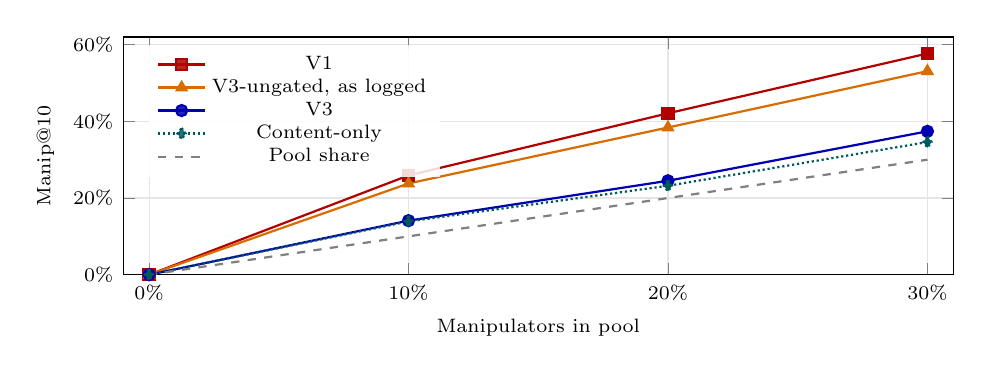
\begin{tikzpicture}
\begin{axis}[width=\columnwidth, height=4.6cm, xlabel={Manipulators in pool}, ylabel={Manip@10},
  xtick={0,0.1,0.2,0.3}, xticklabels={0\%,10\%,20\%,30\%}, ytick={0,0.2,0.4,0.6}, yticklabels={0\%,20\%,40\%,60\%},
  ymin=0, ymax=0.62, xmin=-0.01, xmax=0.31,
  legend pos=north west, legend columns=1, legend style={font=\scriptsize, draw=none, fill=white, fill opacity=0.85, text opacity=1, row sep=-2pt},
  tick label style={font=\scriptsize}, label style={font=\scriptsize}, grid=major, grid style={gray!20}]
\addplot[mark=square*, red!70!black, thick] coordinates {(0,0) (0.1,0.259) (0.2,0.421) (0.3,0.577)};
\addlegendentry{V1}
\addplot[mark=triangle*, orange!85!black, thick] coordinates {(0,0) (0.1,0.238) (0.2,0.384) (0.3,0.531)};
\addlegendentry{V3-ungated, as logged}
\addplot[mark=*, blue!70!black, thick] coordinates {(0,0) (0.1,0.141) (0.2,0.245) (0.3,0.374)};
\addlegendentry{V3}
\addplot[mark=diamond*, teal!70!black, thick, densely dotted] coordinates {(0,0) (0.1,0.139) (0.2,0.232) (0.3,0.346)};
\addlegendentry{Content-only}
\addplot[dashed, gray, thick] coordinates {(0,0) (0.3,0.3)};
\addlegendentry{Pool share}
\end{axis}
\end{tikzpicture}
\caption{Manipulators' share of the top~10 as their share of the pool grows (a separate five-seed run per point). The gated ranker stays close to Content-only, while rankers that trust all logs over-expose manipulators.}
\label{fig:sweep}
\end{figure}

\section{Discussion}
\label{sec:discussion}
\subsection{Relation to Detection}
Proposition~\ref{prop:invariance} guarantees resistance to self-reporting without any simulation, and the experiments show that the gate also improves accuracy over ungated ranking. Manipulator detectors \cite{li2016,fang2018,sundar2020} are complementary: because the gate already removes every unconfirmed record, a detector need only examine the confirmed ones, a far smaller and cleaner set.

\subsection{Design Implications}
Our results suggest three rules for platforms that rank people. First, records written by the ranked party should carry no weight. Second, only verified accounts should be able to confirm records. Third, each counterparty should vouch at most once, which bounds collusion by the number of distinct accomplices and, in our study, also improved accuracy.

\subsection{Validity}
The study uses the platform's own ranking function, 20 paired seeds and Holm-corrected tests, and its conclusions hold across confirmation rates, history depths and collusion strengths. As in prior attack studies \cite{mobasher2007}, the campus generator encodes modelling assumptions; the platform's recommendation logs will allow the same comparisons on live data.

\section{Conclusion}
On mentoring platforms, the candidate being ranked often writes the evidence used to rank them. We studied evidence gating, under which only records that the mentee created or confirmed and annotated may influence rank, stated it as enforceable invariants, and built it into a deployed platform. In a controlled study with the platform's ranking function, the gate removed the damage caused by self-reported history under a fair baseline, neutralised inflators, and gave verified history an advantage over content-only ranking that grew as records accumulated. A one-record-per-mentee cap bounded collusion while improving accuracy. Future work will add exposure control for new mentors, evaluate adaptive attackers and run a campus pilot using the platform's recommendation logs.

\bibliographystyle{IEEEtran}
\bibliography{references}

\end{document}
